\section{Rename Operation}
\hspace*{0.50in} Sampai sekarang, baik Tom dan Jerry menggunakan perintah manual untuk menyusun proyek mereka. Sekarang, Jerry memutuskan untuk membuat Makefile untuk proyek mereka dan juga memberi nama yang tepat untuk file "string.c". \par
\noindent 
{\fontsize{10pt}{10pt}\selectfont [jerry@CentOS project] $  \$  $ pwd} \par
\noindent 
{\fontsize{10pt}{10pt}\selectfont /home/jerry/jerry $  \_  $repo/project} \par
\noindent 
\vspace{10pt}
\noindent 
{\fontsize{10pt}{10pt}\selectfont [jerry@CentOS project] $  \$  $ ls} \par
\noindent 
{\fontsize{10pt}{10pt}\selectfont README src} \par
\noindent 
\vspace{10pt}
\noindent 
{\fontsize{10pt}{10pt}\selectfont [jerry@CentOS project] $  \$  $ cd src/} \par
\noindent 
\vspace{10pt}
\noindent 
{\fontsize{10pt}{10pt}\selectfont [jerry@CentOS src] $  \$  $ git add Makefile} \par
\noindent 
\vspace{10pt}
\noindent 
{\fontsize{10pt}{10pt}\selectfont [jerry@CentOS src] $  \$  $ git mv string.c string $  \_  $operations.c} \par
\noindent 
\vspace{10pt}
\noindent 
{\fontsize{10pt}{10pt}\selectfont [jerry@CentOS src] $  \$  $ git status -s} \par
\noindent 
{\fontsize{10pt}{10pt}\selectfont A Makefile} \par
\noindent 
{\fontsize{10pt}{10pt}\selectfont R string.c  $ - $> string $  \_  $operations.c} \par
\vspace{12pt}
\hspace*{0.50in}Git menunjukkan R sebelum nama file untuk menunjukkan bahwa file telah diganti namanya. \par
\hspace*{0.50in}Untuk komit operasi, Jerry menggunakan - bendera, yang membuat git komit secara otomatis mendeteksi file yang dimodifikasi : \par
\begin{verbatim}
[jerry@CentOS src] $  \$  $ git commit -a -m 'Added 
Makefile and renamed strings.c to string $  \_  
$operations.c ' 

[master 94f7b26] Added Makefile and renamed strings.c to
string $  \_  $operations.c 1 files changed, 0 
insertions(+), 0 deletions(-) 

create mode 100644 src/Makefile 
rename src/ $  \{  $string.c => string $  \_  $operations
.c $  \}  $ (100 $  \%  $)

[jerry@CentOS src] $  \$  $ 
\end{verbatim}

\vspace{12pt}
\noindent 
Perintah di atas akan menghasilkan hasil sebagai berikut: \par
\noindent 
Counting objects: 6, done. \par
\noindent 
Compressing objects: 100 $  \%  $ (3/3), done. \par
\noindent 
Writing objects: 100 $  \%  $ (4/4), 396 bytes, done. \par
\noindent 
Total 4 (delta 0), reused 0 (delta 0) \par
\noindent 
To gituser@git.server.com:project.git \par
\noindent 
7d9ea97..94f7b26 master  $ - $> master \par
\vspace{12pt}
\hspace*{0.50in} Sekarang, pengembang lain dapat melihat modifikasi ini dengan memperbarui repositori lokal mereka. \par
\hspace*{0.50in}Kegunaan utama dari sistem kontrol versi ialah sebagai alat untuk manajemen kode program. Terdapat dua kegunaan utama dari sistem ini, yaitu: \par
\begin{itemize}
\item Menggabungkan perubahan-perubahan kode dari versi lama (misal: untuk mengembalikan fitur yang telah dihapus)

\item Menggabungkan perubahan dari orang lain (misal: menggabungkan fitur yang dikembangkan oleh anggota tim lain)
\end{itemize}
 
\vspace{12pt}
\subsection{Intalasi Git} \par
\hspace*{0.50in} Git berjalan pada semua sistem operasi populer (Mac, Windows, Linux). Jika menggunakan Windows atau Mac, masuk ke situs utama git pada lalu lakukan download dan instalasi software tersebut. Pengguna Linux dapat melakukan instalasi melalui repositori distribusi yang dilakukan, melalui perintah sejenis: \par
\noindent 
{\fontsize{10pt}{10pt}\selectfont yum install git} \par
\vspace{12pt}
\noindent 
pada repositori berbasis RPM, atau perintah : \par
\noindent 
{\fontsize{10pt}{10pt}\selectfont apt-get install git} \par
\vspace{12pt}
\hspace*{0.50in} Untuk repositori berbasis deb. Kembali lagi, perintah hanya diberikan untuk distribusi paling populer (Debian / Ubuntu dan RedHat / Fedora), karena keterbatasan ruang. Jika menggunakan distrusi lain (seperti Gentoo atau Arch, maka diasumsikan telah mengetahui cara instalasi git atau perangkat lunak lain pada umumnya). \par
\hspace*{0.50in} Khusus untuk sistem operasi Windows, pastikan instalasi diambil dari 
, karena pada paket yang tersedia di website tersebut telah diikutkan juga OpenSSH, yang akan sangat berguna jika ingin berkolaborasi dengan programmer lain. Perintah git juga harus memberikan respon yang benar: \par
\noindent 
{\fontsize{10pt}{10pt}\selectfont bert@LYNNSLENIA  $  \sim  $} \par
\noindent 
{\fontsize{10pt}{10pt}\selectfont  $  \$  $ git} \par
\noindent 
{\fontsize{10pt}{10pt}\selectfont usage: git [--version] [--exec-path[=<path>]] [--html-path] [--man-path] [--info-path]} \par
\noindent 
{\fontsize{10pt}{10pt}\selectfont ~~~~~~~~~~ [-p $  \vert  $--paginate $  \vert  $--no-pager] [--no-replace-objects] [--bare]} \par
\noindent 
{\fontsize{10pt}{10pt}\selectfont ~~~~~~~~~~ [--git-dir=<path>] [--work-tree=<path>] [--namespace=<name>]} \par
\noindent 
{\fontsize{10pt}{10pt}\selectfont ~~~~~~~~~~ [-c name=value] [--help]} \par
\noindent 
{\fontsize{10pt}{10pt}\selectfont ~~~~~~~~~~ <command> [<args>]} \par

\subsection{Inisiasi} \par
\hspace*{0.50in} Untuk dapat menggunakan sistem kontrol versi, terlebih dahulu kita harus mempersiapkan repositori. Sebuah repositori menyimpan seluruh versi dari kode program kita. Tidak usah takut, karena repositori tidak akan memakan banyak ruang \emph{hard disk}, karena penyimpanan tidak dilakukan terhadap keseluruhan file. Repositori hanya akan menyimpan \emph{perubahan} yang terjadi pada kode kita dari satu versi ke versi lainnya. Bahasa kerennya, repositori hanya menyimpan delta dari kode pada setiap versinya. \par
\hspace*{0.50in}Pada (di saat kontrol versi yang populer adalah cvs dan programmer pada umumnya berjanggut putih), membangun repositori kode baru adalah hal yang sangat sulit dilakukan. Harus memiliki sebuah \emph{server} khusus yang dapat diakses oleh seluruh anggota tim. Jika server tidak dapat diakses karena jaringan rusak atau internet putus, maka tidak dapat melakukan kontrol versi (dan harus kembali ke metode direktori, atau tidak bekerja). \par
\hspace*{0.50in} Git merupakan sistem kontrol versi terdistribusi, yang berarti git dapat dijalankan tanpa perlu adanya repositori terpusat. Yang diperlukan untuk membuat repositori ialah mengetikkan perintah tertentu di direktori utama. Mulai membuat repositori baru.: \par
\noindent 
{\fontsize{10pt}{10pt}\selectfont bert@LYNNSLENIA  $  \sim  $} \par
\noindent 
{\fontsize{10pt}{10pt}\selectfont  $  \$  $ cd Desktop/projects/git-tutor/} \par
\noindent 
{\fontsize{10pt}{10pt}\selectfont bert@LYNNSLENIA  $  \sim  $/Desktop/projects/git-tutor} \par
\noindent 
{\fontsize{10pt}{10pt}\selectfont  $  \$  $ ls} \par
\noindent 
{\fontsize{10pt}{10pt}\selectfont bert@LYNNSLENIA  $  \sim  $/Desktop/projects/git-tutor} \par
\noindent 
{\fontsize{10pt}{10pt}\selectfont  $  \$  $} \par
\noindent 

\vspace{10pt}
Menambahkan kode baru ke dalam direktori ini.Buat sebuah file baru yang bernama cerita.txt di dalam direktori tersebut: \par
\noindent 
{\fontsize{10pt}{10pt}\selectfont bert@LYNNSLENIA  $  \sim  $/Desktop/projects/git-tutor} \par
\noindent 
{\fontsize{10pt}{10pt}\selectfont  $  \$  $ echo "ini adalah sebuah cerita" > cerita.txt} \par
\noindent 
{\fontsize{10pt}{10pt}\selectfont bert@LYNNSLENIA  $  \sim  $/Desktop/projects/git-tutor} \par
\noindent 
{\fontsize{10pt}{10pt}\selectfont  $  \$  $ ls} \par
\noindent 
{\fontsize{10pt}{10pt}\selectfont cerita.txt} \par
\vspace{12pt}
\noindent 
Kemudian masukkan perintah git init untuk melakukan inisialisasi repositori: \par
\noindent 
{\fontsize{10pt}{10pt}\selectfont bert@LYNNSLENIA  $  \sim  $/Desktop/projects/git-tutor} \par
\noindent 
{\fontsize{10pt}{10pt}\selectfont  $  \$  $ git init} \par
\noindent 
{\fontsize{10pt}{10pt}\selectfont Initialized empty Git repository in c:/Users/bert/Desktop/projects/git-tutor/.git/} \par
\vspace{12pt}
\hspace*{0.50in} Setelah melakukan inisialisasi, git secara otomatis akan membuat direktori .git pada repositori  (lihat potongan kode di bawah). Direktori tersebut merupakan direktori yang digunakan oleh git untuk menyimpan basis data delta kode, dan berbagai metadata lainnya. Mengubah direktori tersebut dapat menyebabkan hilangnya seluruh \emph{history} dari kode. \par
\noindent 
{\fontsize{10pt}{10pt}\selectfont bert@LYNNSLENIA  $  \sim  $/Desktop/projects/git-tutor (master)} \par
\noindent 
{\fontsize{10pt}{10pt}\selectfont  $  \$  $ ls -a} \par
\noindent 
{\fontsize{10pt}{10pt}\selectfont git  cerita.txt} 


\subsection{Penambahan File ke Repository} \par
\hspace*{0.50in} Penyimpanan sejarah dapat dimulai dari saat pertama: kapan file tersebut dibuat dan ditambahkan ke dalam repositori. Untuk menambahkan file ke dalam repositori, gunakan perintah git add: \par

{\fontsize{10pt}{10pt}\selectfont bert@LYNNSLENIA  $  \sim  $/Desktop/projects/git-tutor (master)} \par
{\fontsize{10pt}{10pt}\selectfont  $  \$  $ git add .} \par
{\fontsize{10pt}{10pt}\selectfont warning: LF will be replaced by CRLF in cerita.txt.} \par
{\fontsize{10pt}{10pt}\selectfont The file will have its original line endings in your working directory.} \par
\noindent 
\vspace{12pt}
\noindent 

Secara sederhana, sintaks dari perintah git add adalah sebagai berikut: \par
{\fontsize{10pt}{10pt}\selectfont git add [nama file atau pola]} \par
\noindent 
\vspace{12pt}

\hspace*{0.50in} Memasukkan nama file dalam perintah git add pada dasarnya akan memerintahkan git untuk menambahkan \textbf{semua} file baru dalam repositori. Jika hanya ingin menambahkan satu file (misalkan ada file yang belum yakin akan ditambahkan ke repositori), nama file spesifik dapat dimasukkan: \par
{\fontsize{10pt}{10pt}\selectfont git add cerita.txt} \par

\vspace{12pt}
\hspace*{0.50in}Setelah menambahkan file ke dalam repositori, harus melakukan \emph{commit}. Perintah \emph{commit} memberitahukan kepada git untuk menyimpan sejarah dari file yang telah ditambahkan. Pada git, penambahan, perubahan, ataupun penghapusan sebuah file baru akan tercatat jika perntah \emph{commit} telah dijalankan. Mari lakukan \emph{commit} dengan menjalankan perintah git commit: \par
{\fontsize{10pt}{10pt}\selectfont bert@LYNNSLENIA  $  \sim  $/Desktop/projects/git-tutor (master)} \par
{\fontsize{10pt}{10pt}\selectfont  $  \$  $ git commit} \par
\vspace{12pt}

\hspace*{0.50in} Jika langkah di atas diikuti dengan benar, maka kembali ke {\fontsize{11pt}{11pt}\selectfont git bash, dengan pesan berikut:} \par
{\fontsize{10pt}{10pt}\selectfont bert@LYNNSLENIA  $  \sim  $/Desktop/projects/git-tutor (master)} \par
{\fontsize{10pt}{10pt}\selectfont  $  \$  $ git commit} \par
{\fontsize{10pt}{10pt}\selectfont [master (root-commit) 1d4cdc9] Inisialisasi repo. Penambahan cerita.txt.} \par
{\fontsize{10pt}{10pt}\selectfont warning: LF will be replaced by CRLF in cerita.txt.} \par
{\fontsize{10pt}{10pt}\selectfont The file will have its original line endings in your working directory.} \par
{\fontsize{10pt}{10pt}\selectfont  1 file changed, 1 insertion(+)} \par
{\fontsize{10pt}{10pt}\selectfont  create mode 100644 cerita.txt} \par
\vspace{8pt}

\subsection{ Mengubah Isi File} \par
\hspace*{0.50in}Kegunaan utama kontrol versi (yang tercermin dari namanya) ialah melakukan manajemen perubahan secara otomatis untuk kita. dan kemudian jalankan perintah git commit lagi: \par
{\fontsize{10pt}{10pt}\selectfont bert@LYNNSLENIA  $  \sim  $/Desktop/projects/git-tutor (master)} \par
{\fontsize{10pt}{10pt}\selectfont  $  \$  $ git commit} \par
{\fontsize{10pt}{10pt}\selectfont  $  \#  $ On branch master} \par
{\fontsize{10pt}{10pt}\selectfont  $  \#  $ Changes not staged for commit:} \par
{\fontsize{10pt}{10pt}\selectfont  $  \#  $~~ (use "git add <file>..." to update what will be committed)} \par
{\fontsize{10pt}{10pt}\selectfont  $  \#  $~~ (use "git checkout -- <file>..." to discard changes in working directory)} \par
{\fontsize{10pt}{10pt}\selectfont  $  \#  $} \par
{\fontsize{10pt}{10pt}\selectfont  $  \#  $~~~~~~~modified:~  cerita.txt} \par
{\fontsize{10pt}{10pt}\selectfont  $  \#  $} \par
{\fontsize{10pt}{10pt}\selectfont no changes added to commit (use "git add" and/or "git commit -a")} \par
\vspace{12pt}
\hspace*{0.50in}Perhatikan bahwa git secara otomatis mengetahui file mana saja yang berubah, tetapi tidak melakukan pencatatan perubahan tersebut. Untuk memerintahkan git mencatat perubahan tersebut, gunakan perintah git commit -a: \par
{\fontsize{10pt}{10pt}\selectfont bert@LYNNSLENIA  $  \sim  $/Desktop/projects/git-tutor (master)} \par
{\fontsize{10pt}{10pt}\selectfont  $  \$  $ git commit -a} \par
{\fontsize{10pt}{10pt}\selectfont [master 61c4707] Kapitalisasi dan melengkapi kalimat.} \par
{\fontsize{10pt}{10pt}\selectfont  1 file changed, 1 insertion(+), 1 deletion(-)} \par
\vspace{12pt}
\hspace*{0.50in}Selain melakukan perubahan, tentunya terkadang kita ingin mengetahui perubahan-perubahan apa saja yang terjadi selama pengembangan. Untuk melihat daftar perubahan yang telah dilakukan, kita dapat menggunakan perintah git log: \par
\noindent 
{\fontsize{10pt}{10pt}\selectfont bert@LYNNSLENIA  $  \sim  $/Desktop/projects/git-tutor (master)} \par
\noindent 
{\fontsize{10pt}{10pt}\selectfont  $  \$  $ git log} \par
\noindent 
{\fontsize{10pt}{10pt}\selectfont commit 61c47074ee583dbdd16fa9568019e80d864fb403} \par
\noindent 
{\fontsize{10pt}{10pt}\selectfont Author: Alex Xandra Albert Sim <bertzzie@gmail.com>} \par
\noindent 
{\fontsize{10pt}{10pt}\selectfont Date:~~ Sun Dec 23 16:36:46 2012 +0700} \par
\noindent 
{\fontsize{10pt}{10pt}\selectfont commit 1d4cdc9350570230d352ef19aededf06769b0698} \par
\noindent 
{\fontsize{10pt}{10pt}\selectfont Author: Alex Xandra Albert Sim <bertzzie@gmail.com>} \par
\noindent 
{\fontsize{10pt}{10pt}\selectfont Date:~~ Sun Dec 23 16:10:33 2012 +0700} \par
\noindent 
\vspace{10pt}
\noindent 
{\fontsize{10pt}{10pt}\selectfont ~~~ Inisialisasi repo. Penambahan cerita.txt.} \par
\vspace{12pt}
\noindent 
Jalankan perintah git log sekali lagi, untuk melihat hasil pekerjaan kita sejauh ini: \par
\noindent 
{\fontsize{10pt}{10pt}\selectfont bert@LYNNSLENIA  $  \sim  $/Desktop/projects/git-tutor (master)} \par
\noindent 
{\fontsize{10pt}{10pt}\selectfont  $  \$  $ git log} \par
\noindent 
{\fontsize{10pt}{10pt}\selectfont commit 28dabb1c54a086cce567ecb890b10339416bcbfa} \par
\noindent 
{\fontsize{10pt}{10pt}\selectfont Author: Alex Xandra Albert Sim <bertzzie@gmail.com>} \par
\noindent 
{\fontsize{10pt}{10pt}\selectfont Date:~~ Sun Dec 23 16:49:21 2012 +0700} \par
\noindent 
{\fontsize{10pt}{10pt}\selectfont commit 61c47074ee583dbdd16fa9568019e80d864fb403} \par
\noindent 
{\fontsize{10pt}{10pt}\selectfont Author: Alex Xandra Albert Sim <bertzzie@gmail.com>} \par
\noindent 
{\fontsize{10pt}{10pt}\selectfont Date:~~ Sun Dec 23 16:36:46 2012 +0700} \par
\noindent 
{\fontsize{10pt}{10pt}\selectfont commit 1d4cdc9350570230d352ef19aededf06769b0698} \par
\noindent 
{\fontsize{10pt}{10pt}\selectfont Author: Alex Xandra Albert Sim <bertzzie@gmail.com>} \par
\noindent 
{\fontsize{10pt}{10pt}\selectfont Date:~~ Sun Dec 23 16:10:33 2012 +0700} \par
\noindent 

\vspace{12pt}
\hspace*{0.50in} Git memungkinkan kita untuk mengembalikan kode ke dalam keadaan sebelumnya, yaitu \emph{commit} terakhir. Melakukan pengembalian kode ini dengan menggunakan perintah git checkout seperti berikut: \par
\noindent 
bert@LYNNSLENIA  $  \sim  $/Desktop/projects/git-tutor (master) \par
\noindent 
 $  \$  $ git checkout HEAD -- cerita.txt \par
\noindent 
bert@LYNNSLENIA  $  \sim  $/Desktop/projects/git-tutor (master) \par
\noindent 
 $  \$  $ ls \par
\noindent 
cerita.txt \par
\noindent 
bert@LYNNSLENIA  $  \sim  $/Desktop/projects/git-tutor (master) \par
\noindent 
 $  \$  $ cat cerita.txt \par
\noindent 
Ini adalah sebuah cerita tentang seekor kera yang terkurung dan terpenjara dalam goa. \par
\noindent 
Kera ini bernama Sun Go Kong. Dari manakah Sun Go Kong berasal? \par
\noindent 
bert@LYNNSLENIA  $  \sim  $/Desktop/projects/git-tutor (master) \par
\vspace{12pt}
\hspace*{0.50in} Parameter HEAD pada perintah yang kita jalankan merupakan parameter untuk memberitahukan git checkout bahwa kita ingin mengembalikan kode pada revisi terakhir (HEAD dalam istilah git). Karena hanya ingin mengembalikan file cerita.txt, maka kita harus memberitahukan git checkout, melalui parameter -- cerita.txt. Perintah git checkout juga memiliki banyak kegunaan lainnya selain mengembalikan kode ke revisi tertentu.  \par
\hspace*{0.50in} Untuk melihat bagaimana fitur ini bekerja, mari lakukan perubahan pada repositori terlebih dahulu. Tambahkan sebuah file baru ke dalam repositori: \par
\noindent 
{\fontsize{10pt}{10pt}\selectfont bert@LYNNSLENIA  $  \sim  $/Desktop/projects/git-tutor (master)} \par
\noindent 
{\fontsize{10pt}{10pt}\selectfont  $  \$  $ ls} \par
\noindent 
{\fontsize{10pt}{10pt}\selectfont cerita.txt} \par
\noindent 
\vspace{10pt}
\noindent 
{\fontsize{10pt}{10pt}\selectfont bert@LYNNSLENIA  $  \sim  $/Desktop/projects/git-tutor (master)} \par
\noindent 
{\fontsize{10pt}{10pt}\selectfont  $  \$  $ echo "Seekor kera, terpuruk, terpenjara dalam goa. Di gunung suci sunyi} \par
\noindent 
{\fontsize{10pt}{10pt}\selectfont tempat hukuman para dewa." > lagu-intro.txt} \par
\noindent 
\vspace{10pt}
\noindent 
{\fontsize{10pt}{10pt}\selectfont bert@LYNNSLENIA  $  \sim  $/Desktop/projects/git-tutor (master)} \par
\noindent 
{\fontsize{10pt}{10pt}\selectfont  $  \$  $ ls} \par
\noindent 
{\fontsize{10pt}{10pt}\selectfont cerita.txt~ lagu-intro.txt} \par
\noindent 
\vspace{10pt}
\noindent 
{\fontsize{10pt}{10pt}\selectfont bert@LYNNSLENIA  $  \sim  $/Desktop/projects/git-tutor (master)} \par
\noindent 
{\fontsize{10pt}{10pt}\selectfont  $  \$  $ git add .} \par
\noindent 
{\fontsize{10pt}{10pt}\selectfont warning: LF will be replaced by CRLF in lagu-intro.txt.} \par
\noindent 
{\fontsize{10pt}{10pt}\selectfont The file will have its original line endings in your working directory.} \par
\noindent 
\vspace{10pt}
\noindent 
{\fontsize{10pt}{10pt}\selectfont bert@LYNNSLENIA  $  \sim  $/Desktop/projects/git-tutor (master)} \par
\noindent 
{\fontsize{10pt}{10pt}\selectfont  $  \$  $ git commit} \par
\noindent 
{\fontsize{10pt}{10pt}\selectfont [master 03d0628] Penambahan lagu intro.} \par
\noindent 
{\fontsize{10pt}{10pt}\selectfont warning: LF will be replaced by CRLF in lagu-intro.txt.} \par
\noindent 
{\fontsize{10pt}{10pt}\selectfont The file will have its original line endings in your working directory.} \par
\noindent 
{\fontsize{10pt}{10pt}\selectfont  1 file changed, 1 insertion(+)} \par
\noindent 
{\fontsize{10pt}{10pt}\selectfont  create mode 100644 lagu-intro.txt} \par
\vspace{12pt}
\hspace*{0.50in} Kemudian kita akan melakukan edit terhadap cerita.txt dan mengganti nama lagu-intro.txt menjadi lagu-intro-awal.txt: \par
\begin{verbatim}
ert@LYNNSLENIA  $  \sim  $/Desktop/projects/git-tutor 
(master) 
 $  \$  $ ls \par
cerita.txt~ lagu-intro.txt \par
bert@LYNNSLENIA  $  \sim  $/Desktop/projects/git-tutor 
(master) 
 $  \$  $ notepad cerita.txt \par
bert@LYNNSLENIA  $  \sim  $/Desktop/projects/git-tutor 
(master) 
 $  \$  $ mv lagu-intro.txt lagu-intro-awal.txt 
bert@LYNNSLENIA  $  \sim  $/Desktop/projects/git-tutor 
(master) 
$  \$  $ ls 
cerita.txt lagu-intro-awal.txt 
\end{verbatim}

\hspace*{0.50in} Setelah melakukan perubahan tersebut, kita mengalami amnesia sesaat karena kucing kantor jatuh ke kepala kita (kucing yang menyebalkan!). Karena telah lupa akan perubahan yang dilakukan, kita dapat melihat apa saja yang berubah dengan menggunakan perintah git status: \par
\noindent 
{\fontsize{10pt}{10pt}\selectfont bert@LYNNSLENIA  $  \sim  $/Desktop/projects/git-tutor (master)} \par
\noindent 
{\fontsize{10pt}{10pt}\selectfont  $  \$  $ git status} \par
\noindent 
{\fontsize{10pt}{10pt}\selectfont  $  \#  $ On branch master} \par
\noindent 
{\fontsize{10pt}{10pt}\selectfont  $  \#  $ Changes not staged for commit:} \par
\noindent 
{\fontsize{10pt}{10pt}\selectfont  $  \#  $~~ (use "git add/rm <file>..." to update what will be committed)} \par
\noindent 
{\fontsize{10pt}{10pt}\selectfont  $  \#  $~~ (use "git checkout -- <file>..." to discard changes in working directory)} \par
\noindent 
{\fontsize{10pt}{10pt}\selectfont  $  \#  $} \par
\noindent 
{\fontsize{10pt}{10pt}\selectfont  $  \#  $~~~~~~~modified:~  cerita.txt} \par
\noindent 
{\fontsize{10pt}{10pt}\selectfont  $  \#  $~~~~~~~deleted:~~  lagu-intro.txt} \par
\noindent 
{\fontsize{10pt}{10pt}\selectfont  $  \#  $} \par
\noindent 
{\fontsize{10pt}{10pt}\selectfont  $  \#  $ Untracked files:} \par
\noindent 
{\fontsize{10pt}{10pt}\selectfont  $  \#  $~~ (use "git add <file>..." to include in what will be committed)} \par
\noindent 
{\fontsize{10pt}{10pt}\selectfont  $  \#  $} \par
\noindent 
{\fontsize{10pt}{10pt}\selectfont  $  \#  $~~~~~~ lagu-intro-awal.txt} \par
\noindent 
{\fontsize{10pt}{10pt}\selectfont no changes added to commit (use "git add" and/or "git commit -a")} \par
\vspace{12pt}
\noindent 
\hspace*{0.50in} $ " $Changes not staged for commit $ " $ menampilkan daftar file yang berubah, tetapi belum di-\textit{commit}. File yang tercatat ini termasuk file yang diubah dan dihapus. \par
\noindent 
$ " $Untracked files $ " $ menampilkan file yang belum ditambahkan ke dalam repositori.
 \par
\noindent 
Jika ingin melihat apa saja yang diubah pada file {\fontsize{10pt}{10pt}\selectfont cerita.txt, kita dapat menggunakan perintah git diff:} \par
\noindent 
{\fontsize{10pt}{10pt}\selectfont bert@LYNNSLENIA  $  \sim  $/Desktop/projects/git-tutor (master)} \par
\noindent 
{\fontsize{10pt}{10pt}\selectfont  $  \$  $ git diff cerita.txt} \par
\noindent 
{\fontsize{10pt}{10pt}\selectfont diff --git a/cerita.txt b/cerita.txt} \par
\noindent 
{\fontsize{10pt}{10pt}\selectfont index 846114d..dbcb596 100644} \par
\noindent 
{\fontsize{10pt}{10pt}\selectfont --- a/cerita.txt} \par
\noindent 
{\fontsize{10pt}{10pt}\selectfont +++ b/cerita.txt} \par
\noindent 
{\fontsize{10pt}{10pt}\selectfont @@ -1,3 +1,3 @@} \par
\noindent 
{\fontsize{10pt}{10pt}\selectfont  Ini adalah sebuah cerita tentang seekor kera yang terkurung dan terpenjara dala} \par
\noindent 
\vspace{10pt}
\noindent 
{\fontsize{10pt}{10pt}\selectfont -Kera ini bernama Sun Go Kong. Dari manakah Sun Go Kong berasal?} \par
\noindent 
{\fontsize{10pt}{10pt}\selectfont +Kera ini bernama Sun Go Kong. Dari manakah Sun Go Kong berasal???!} \par
\noindent 
{\fontsize{10pt}{10pt}\selectfont (END)} \par
\vspace{12pt}
\hspace*{0.50in} Format yang ditampilkan mungkin agak membingungkan, tetapi tidak usah takut, karena bagian yang perlu diperhatikan hanyalah pada bagian yang bertanda - dan +. Pada git bash, bahkan bagian ini diberi warna (merah untuk - dan hijau untuk +). Tanda +, tentunya berarti bagian yang ditambahkan, dan tanda - berarti bagian yang dihapus. Dengan melihat perubahan pada baris yang bersangkutan, kita dapat mengetahui bahwa ? diubah menjadi ???! pada akhir baris. \par
\hspace*{0.50in} Setelah mengetahui perubahan yang dilakukan, dan menganggap perubahan tersebut aman untuk di-\emph{commit}, kita lalu dapat melakukan \emph{commit} seperti biasa: \par
{\fontsize{10pt}{10pt}\selectfont bert@LYNNSLENIA  $  \sim  $/Desktop/projects/git-tutor (master)} \par
{\fontsize{10pt}{10pt}\selectfont  $  \$  $ git add lagu-intro-awal.txt} \par
{\fontsize{10pt}{10pt}\selectfont warning: LF will be replaced by CRLF in lagu-intro-awal.txt.} \par
{\fontsize{10pt}{10pt}\selectfont The file will have its original line endings in your working directory.} \par
\vspace{10pt}
{\fontsize{10pt}{10pt}\selectfont bert@LYNNSLENIA  $  \sim  $/Desktop/projects/git-tutor (master)} \par
{\fontsize{10pt}{10pt}\selectfont  $  \$  $ git commit} \par
{\fontsize{10pt}{10pt}\selectfont [master 306f422] Dramatisasi cerita dan perubahan nama file lagu.} \par
{\fontsize{10pt}{10pt}\selectfont warning: LF will be replaced by CRLF in lagu-intro-awal.txt.} \par
{\fontsize{10pt}{10pt}\selectfont The file will have its original line endings in your working directory.} \par
{\fontsize{10pt}{10pt}\selectfont  1 file changed, 1 insertion(+)} \par
{\fontsize{10pt}{10pt}\selectfont  create mode 100644 lagu-intro-awal.txt} \par
\vspace{10pt}
{\fontsize{10pt}{10pt}\selectfont bert@LYNNSLENIA  $  \sim  $/Desktop/projects/git-tutor (master)} \par
{\fontsize{10pt}{10pt}\selectfont  $  \$  $ git log} \par
{\fontsize{10pt}{10pt}\selectfont commit 306f42258f4bfee95d10396777391ae013bc6edd} \par
{\fontsize{10pt}{10pt}\selectfont Author: Alex Xandra Albert Sim <bertzzie@gmail.com>} \par
{\fontsize{10pt}{10pt}\selectfont Date:~~ Sun Dec 23 18:22:30 2012 +0700} \par
\vspace{10pt}
{\fontsize{10pt}{10pt}\selectfont ~~~ Dramatisasi cerita dan perubahan nama file lagu.} \par
\vspace{10pt}
{\fontsize{10pt}{10pt}\selectfont commit 03d06284462f7fc43b610d522678f4f22cdd9a40} \par
{\fontsize{10pt}{10pt}\selectfont Author: Alex Xandra Albert Sim <bertzzie@gmail.com>} \par
{\fontsize{10pt}{10pt}\selectfont Date:~~ Sun Dec 23 18:08:10 2012 +0700} \par
\vspace{10pt}
{\fontsize{10pt}{10pt}\selectfont ~~~ Penambahan lagu intro.} \par
\vspace{10pt}
{\fontsize{10pt}{10pt}\selectfont commit 28dabb1c54a086cce567ecb890b10339416bcbfa} \par
{\fontsize{10pt}{10pt}\selectfont Author: Alex Xandra Albert Sim <bertzzie@gmail.com>} \par
{\fontsize{10pt}{10pt}\selectfont Date:~~ Sun Dec 23 16:49:21 2012 +0700} \par
\vspace{10pt}
{\fontsize{10pt}{10pt}\selectfont ~~~ Penambahan misteri terbesar di dunia.} \par
\vspace{10pt}
{\fontsize{10pt}{10pt}\selectfont commit 61c47074ee583dbdd16fa9568019e80d864fb403} \par
{\fontsize{10pt}{10pt}\selectfont Author: Alex Xandra Albert Sim <bertzzie@gmail.com>} \par
{\fontsize{10pt}{10pt}\selectfont Date:~~ Sun Dec 23 16:36:46 2012 +0700} \par
\vspace{10pt}
{\fontsize{10pt}{10pt}\selectfont ~~~ Kapitalisasi dan melengkapi kalimat.} \par
\vspace{10pt}
{\fontsize{10pt}{10pt}\selectfont commit 1d4cdc9350570230d352ef19aededf06769b0698} \par
{\fontsize{10pt}{10pt}\selectfont Author: Alex Xandra Albert Sim <bertzzie@gmail.com>} \par
{\fontsize{10pt}{10pt}\selectfont Date:~~ Sun Dec 23 16:10:33 2012 +0700} \par
\vspace{10pt}
{\fontsize{10pt}{10pt}\selectfont ~~~ Inisialisasi repo. Penambahan cerita.txt.} 

\subsection{Membaca File Lama, dan Menjalankan Mesin Waktu}
\hspace*{0.50in} Nomor revisi, seperti yang telah dijelaskan sebelumnya, berguna sebagai tanda untuk memisahkan antara satu \emph{commit} dengan \emph{commit} lainnya. Misalnya jika  ingin melihat isi file cerita.txt pada saat awal pertama kali dibuat, kita dapat menggunakan perintah git show, yang sintaksnya adalah: \par
git show [nomor revisi]:[nama file] \par
\vspace{12pt}
\noindent 
contoh pengunaan: \par
bert@LYNNSLENIA  $  \sim  $/Desktop/projects/git-tutor (master) \par
 $  \$  $ git show 1d4cdc:cerita.txt \par
ini adalah sebuah cerita \par
\vspace{12pt}
\hspace*{0.50in} Perhatikan bahwa nomor commit yang dimasukkan hanyalah enam karakter saja. Jika keenam karakter tersebut sama untuk beberapa nomor \textit{commit}, kita baru perlu memasukkan karakter selanjutnya, sampai tidak terdapat konflik nama lagi. \par
\hspace*{0.50in} Sesuai dengan nomor revisi dengan menggunakan {\fontsize{10pt}{10pt}\selectfont git checkcout yang telah dijelaskan sebelumnya. Contohnya :} \par
bert@LYNNSLENIA  $  \sim  $/Desktop/projects/git-tutor (master) \par
 $  \$  $ ls \par
cerita.txt~ lagu-intro-awal.txt \par
\vspace{12pt}
bert@LYNNSLENIA  $  \sim  $/Desktop/projects/git-tutor (master) \par
 $  \$  $ cat cerita.txt \par
Ini adalah sebuah cerita tentang seekor kera yang terkurung dan terpenjara dalam \par
 goa. \par
\vspace{12pt}
Kera ini bernama Sun Go Kong. Dari manakah Sun Go Kong berasal???! \par
\vspace{12pt}
bert@LYNNSLENIA  $  \sim  $/Desktop/projects/git-tutor (master) \par
 $  \$  $ git checkout 61c470 cerita.txt \par
\vspace{12pt}
bert@LYNNSLENIA  $  \sim  $/Desktop/projects/git-tutor (master) \par
 $  \$  $ cat cerita.txt \par
Ini adalah sebuah cerita tentang seekor kera yang terkurung dan terpenjara dalam \par
 goa. \par
bert@LYNNSLENIA  $  \sim  $/Desktop/projects/git-tutor (master) \par
 $  \$  $ git checkout 1d4cdc cerita.txt \par
\vspace{12pt}
bert@LYNNSLENIA  $  \sim  $/Desktop/projects/git-tutor (master) \par
 $  \$  $ cat cerita.txt \par
ini adalah sebuah cerita \par
\vspace{12pt}
bert@LYNNSLENIA  $  \sim  $/Desktop/projects/git-tutor (master) \par
 $  \$  $ git checkout 03d0628 cerita.txt \par
\vspace{12pt}
bert@LYNNSLENIA  $  \sim  $/Desktop/projects/git-tutor (master) \par
 $  \$  $ cat cerita.txt \par
Ini adalah sebuah cerita tentang seekor kera yang terkurung dan terpenjara dalam \par
 goa. \par
\vspace{12pt}
Kera ini bernama Sun Go Kong. Dari manakah Sun Go Kong berasal? \par
bert@LYNNSLENIA  $  \sim  $/Desktop/projects/git-tutor (master) \par
 $  \$  $ git checkout HEAD cerita.txt \par
\vspace{12pt}
bert@LYNNSLENIA  $  \sim  $/Desktop/projects/git-tutor (master) \par
 $  \$  $ cat cerita.txt \par
Ini adalah sebuah cerita tentang seekor kera yang terkurung dan terpenjara dalam \par
 goa. \par
\vspace{12pt}
Kera ini bernama Sun Go Kong. Dari manakah Sun Go Kong berasal???! \par
\vspace{11pt}
\noindent 
{\fontsize{11pt}{11pt}\selectfont  \hspace*{0.50in} Perhatikan bahwa pada saat menggunakan perintah git checkout, menggunakan cat untuk melihat isi file. Hal ini dikarenakan git checkout benar-benar mengubah file yang ada pada repositori, berbeda dengan git show yang hanya menampilkan file tersebut pada revisi tertentu.} \par

\section{Penyelesaian Masalah}
\hspace*{0.5in} Mengalami kesalahan ini saat mencoba mengganti nama remote. Tidak bisa mengganti nama config section 'remote [nama lama]' ke 'remote [nama baru] kesalahan ini berarti remote yang dicoba dengan nama remote lama yang diketik tidak ada. Memeriksa remote yang ada saat ini dengan perintah \ref{Penamaan} Penamaan Remote git remote -v:
\begin{figure}[ht]
	\centerline{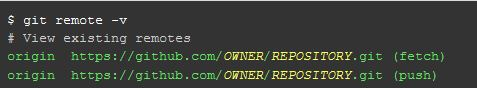
\includegraphics[width=0.70\textwidth]{Figures/Penamaan}}
	\caption{Penamaan}
	\label{Penamaan}
\end{figure}

\hspace*{0.5in} Kesalahan ini berarti nama remote yang ingin digunakan sudah ada. Untuk mengatasi ini, gunakan nama jauh yang berbeda, atau ganti nama remote asli.
